\documentclass[thesis.tex]{subfiles}

\chapter{Bài toán xác minh người nói}

\section{Nhận dạng người nói}

Nhận dạng người nói (speaker recognition) là quá trình tự động nhận dạng người đang nói bằng cách sử dụng thông tin riêng biệt của người nói đó có trong tín hiệu âm thanh. Nhận dạng người nói được ứng dụng rộng rãi trong nhiều lĩnh vực khác nhau, tuy nhiên cũng gặp không ít khó khăn khi triển khai trong thực tế. Do vây, nghiên cứu bài toán nhận dạng người nói rất được quan tâm bởi nhiều nhà khoa học trên thế giới. Một số ứng dụng của bài toán có thể kể đến như:

\begin{itemize}
    \item Bảo mật cho các hệ thống tài chính, ngân hàng: người dùng dùng giọng nói kết hợp với các lớp bảo mật khác cho xác thực để tăng tính bảo mật khi giao dịch.
    \item Tăng trải nghiệm khách hàng trong tổng đài chăm sóc khách hàng.
    \item Xác định danh tính tội phạm trong an ninh khi thu được dữ liệu giọng nói.
    \item Kết hợp với các hệ thống nhận dạng tiếng nói để xây dựng ứng dụng gỡ băng cuộc họp.
    \item ...
\end{itemize}

Dựa vào ứng dụng, nhận dạng người được phân loại thành xác định người nói (speaker identitfication) và xác minh người nói (speaker verfication) (Hình \ref{fig:verification-identification}). Trong xác định người nói, một đoạn tiếng nói từ một người không xác định được phân tích và so sánh với mô hình giọng nói của những người đã biết. Người này được xác định là người mô hình giọng nói phù hợp nhất với câu nói đầu vào. Trong xác minh người nói, một người lạ xác nhận một danh tính đã biết; đoạn tiếng nói của người này được so sánh với mô hình giọng nói của danh tính đang được xác nhận. Nếu điểm tương đồng đủ tốt, nghĩa là trên một ngưỡng nào đó, danh tính của người lạ được chấp nhận. Ngưỡng cao khiến những kẻ mạo danh khó được chấp nhận bởi hệ thống, nhưng có nguy từ chối nhầm người dùng hợp lệ. Ngược lại, ngưỡng thấp cho phép chấp nhận người dùng hợp lệ một cách nhất quán, nhưng có nguy cơ chấp nhận những người giả mạo. 

\begin{figure}[h]
    \centering
    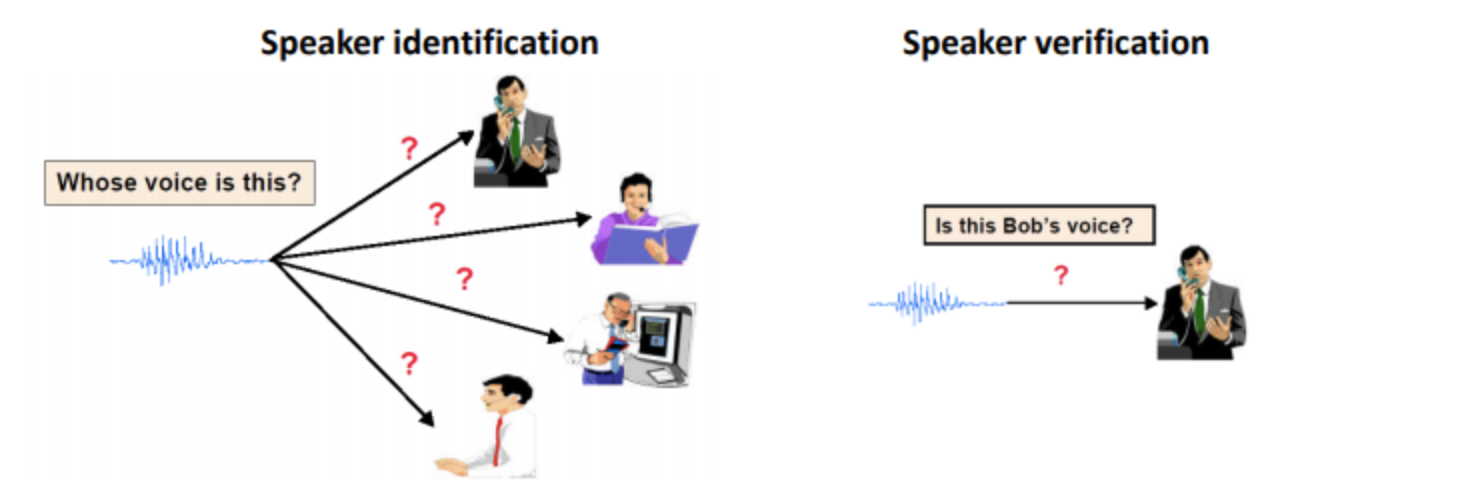
\includegraphics[width=1.0\textwidth]{images/identification-verification.png}
    \caption{Nhận định người nói và xác minh người nói \protect\footnotemark}
    \label{fig:verification-identification}
\end{figure}
\footnotetext{https://wiki.aalto.fi/display/ITSP/Speaker+Recognition+and+Verification}


Thông thường, hệ thống nhận dạng người nói được chia thành 3 pha như mô tả trong Hình \ref*{fig:overall-system}

\begin{itemize}
    \item Pha 1: phát triển (development). Trong pha này, mô hình có khả năng biểu diễn đặc trưng người nói được huấn luyện và tối ưu trên một cơ sở dữ liệu các đoạn tiếng nói từ một nhóm các người nói khác nhau.
    \item Pha 2: ghi danh (enrollment). Trong pha ghi danh, biểu diễn của người dùng mới được trích xuất bằng mô hình phát triển ở pha 1 và lưu trữ trong cơ sở dữ liệu để phục vụ cho pha 3.
    \item Pha 3: kiểm tra (testing). Với bài toán nhận định người nói, vec-tơ biểu diễn của câu nói đầu vào được so sánh với tất cả biểu diễn trong cơ sở dữ liệu để tìm ra người dùng tương đồng nhất. Trong bài toán xác thực người nói, được cung cấp danh tính đầu vào, hệ thống chỉ so sánh đoạn tiếng nói đầu vào và đoạn của danh tính trong hệ thống để đưa ra quyết định.
\end{itemize}

Trong thực tế, hiệu năng của hệ thống nhận diện người nói bị suy giảm do sự khác biệt của các kênh và phiên giữa tín hiệu giọng nói trong pha ghi danh và pha kiểm tra. Các yếu tố làm ảnh hưởng tới tín hiệu giọng nói bao gồm:

\begin{itemize}
    \item Sử dụng các loại micrô khác nhau khi thu tín hiệu đăng ký và kiểm tra.
    \item Điều kiện tiếng ồn và độ vang của môi trường.
    \item Sự khác biệt trong giọng nói của người nói ở các giai đoạn khác nhau của độ tuổi, sức khoẻ, phong cách nói và trạng thái cảm xúc.
    \item Các kênh truyền như các loại điện thoại di động khác nhau, micrô, giao thức truyền âm thanh qua internet có thể làm thay đổi giọng nói.
\end{itemize}

\begin{figure}[h]
    \centering
    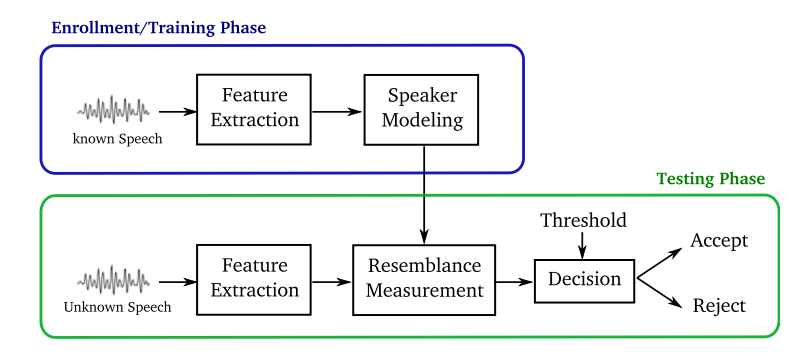
\includegraphics[width=1.0\textwidth]{images/overall-system.png}
    \caption{Tổng quan hệ thống nhận diện người nói}
    \label{fig:overall-system}
\end{figure}

Dựa vào sự tương đồng của các câu nói đầu vào, phương pháp giải quyết bài toán nhận dạng người nói còn có thể chia thành nhóm phụ thuộc văn bản (text-dependent speaker recognition - TDSR) và nhóm không phụ thuộc văn bản(text-independent speaker recognition - TISR). Các hệ thống TDSR yêu cầu người nói cung cấp các đoạn tiếng nói có nội dung theo một từ hoặc câu được định sẵn; nội dung các câu nói phải được giữ nhất quán trong cả quá trình huấn luyện và nhận dạng. Ngược lại, TISR không yêu cầu người dùng phải thu theo bất cứ một văn bản nào. Với các đoạn tiếng nói ngắn, các hệ thống TDSR đã có thể đạt được hiệu suất nhận diện cao, trong khi các TISR yêu cầu các câu nói dài để huấn luyện các mô hình đáng tin cậy và đạt được hiệu suất tốt. Do sự bất tiện của các hệ thống TDSR, trong vài năm gần đây, cộng đồng nghiên cứu tập trung phát triển các mô hình học sâu cho bài toán TISR.

\section{Xác minh người nói trên thế giới}
\TODO{Tình hình nghiên cứu bài toán xác minh người nói trên thế giới}

\section{Xác minh người nói trong tiếng Việt và các vấn đề đặt ra} \label{vietnamese-speaker-recognition}
Ở Việt Nam trong những năm vừa qua, nhờ vào sự phát triển của ngành công nghệ thông tin cũng như sự phát triển mạnh mẽ của nền kinh tế đã tạo điều kiện nghiên cứu, phát triển và triển khai các ứng dụng công nghệ mang lại  nhiều lợi ích cho xã hội. Các ứng dụng trí tuệ nhân tạo như nhận dạng khuôn mặt, nhận dạng giọng nói cũng không nằm ngoài xu thế. Tuy nhiên, theo hiểu biết của tác giả, các nghiên cứu về nhận dạng người nói tiếng Việt hay dữ liệu công khai cho bài toán còn rất hạn chế.

Năm 2010, luận án tiến sĩ của TS. Ngô Minh Dũng \footnote{\href{http://luanan.nlv.gov.vn/luanan?a=d\&d=TTcFabDIJkxi2010.1.5\#}{http://luanan.nlv.gov.vn/luanan?a=d\&d=TTcFabDIJkxi2010.1.5\#}} nghiên cứu giải quyết bài toán nhận dạng người nói tiếng Việt phụ thuộc văn bản. Nghiên cứu xây dựng cơ sở dữ liệu với 150 người nói với 17 âm tiết khác nhau bao gồm 10 âm tiết số và 7 âm tiết khác để thử nghiệm. Luận án sử dụng mô hình Gaussian  hỗn hợp nhằm mô tả phân phân bố tần số cộng hưởng của tuyến phát âm để mô tả người nói. Nghiên cứu \cite{haspeaker, 7054126} bởi các trường Đại học Sư phạm Huế, Đại học Sư phạm Kỹ thuật Hưng Yên và Đại học Bách khoa Hà Nội cùng giải quyết bài toán nhận dạng người nói phụ thuộc văn bản sử dụng mô hình Gaussian hỗn hợp. Nghiên cứu đầu tiên áp dụng học sâu cho bài toán nhận dạng người nói tiếng Việt phụ thuộc văn bản được công bố tại hội nghị SoICT lần thứ 9 vào năm 2018 \cite{nguyen2018vietnamese}. Hiện tại chưa có nghiên cứu hay hệ thống thương mại nào cho nhận diện người nói không phụ thuộc văn bản trong tiếng Việt.

Các mô hình nhận dạng người nói không phụ thuộc văn bản tuy thuận tiện khi sử dụng nhưng để xây dựng mô hình chất lượng tốt cần một lượng dữ liệu khổng lồ. Bộ dữ liệu VoxCeleb thường được sử để xây dựng các mô hình tiếng Anh VoxCeleb có hơn 7,000 danh tính khác nhau, hơn 1,000,000 đoạn âm thanh với tổng độ dài hơn 2,000 giờ. Bộ dữ liệu công khai duy nhất trong tiếng Việt phục vụ cho bài toán không phụ thuộc văn bản được xây dựng cho cuộc thi ZaloAI challenge \cite{ZaloAIChallenge} bao gồm 400 danh tính, 10,000 đoạn âm thanh với tổng độ dài 8.7 giờ, ít hơn rất nhiều so với bộ dữ liệu tiếng Anh. Với lượng dữ liệu nhỏ, việc xây dựng mô hình chất lượng tốt cho tiếng Việt trở nên rất khó khăn.
% https://drive.google.com/file/d/1Qcd7QBRLkMCIJT7pVHy-yDKHLhtHcju1/view

\section{Mục tiêu của đồ án}
Như đã đề cập trong các mục trước, nhận dạng người nói không phụ thuộc văn bản có tính ứng dụng cao và thuận tiện hơn phụ thuộc văn bản. Tuy nhiên, các hệ thống thống kê truyền thống lại không đáp ứng được về mặt hiệu suất. Các phương pháp học sâu hiện đại áp dụng cho bài toán có kết quả tốt nhưng lại yêu cầu một lượng dữ liệu rất lớn.

Để giải quyết việc thiếu hụt dữ liệu phục vụ cho huấn luyện mô hình, tác tác giả bổ sung dữ liệu danh tính bằng hai bộ dữ liệu nhận dạng tiếng nói là VIVOS và VLSP. Ngoài ra nhận thấy bộ dữ liệu còn nhiều lỗi, tác giả cũng xây dựng một bộ lọc dữ liệu dựa trên biểu diễn người nói từ mô hình giúp loại bỏ các đoạn âm thanh không hợp lệ, loại bỏ hay hợp nhất danh tính dễ dàng hơn từ đó tăng chất lượng bộ dữ liệu.

Trong khuôn khổ đồ án, tác giả tập trung vào thử nghiệm các kĩ thuật huấn luyện mô hình học sâu cho nhận dạng người nói tiếng Việt không phụ thuộc văn bản. 

\section{Bố cục đồ án}
Trong chương 1, tác giả đã giới thiệu tổng quan về bài toán nhận dạng người nói, thảo luận về tình hình phát triển nhận dạng người nói trong tiếng Việt. Phần còn lại của đồ án được tổ chức như sau.

Chương 2 trình bày về cơ sở lý thuyết về học máy và học sâu, một số hàm mất mát cơ bản và phương pháp trích xuất đặc trưng từ tín hiệu âm thanh.

Chương 3 trình bày về tình hình nghiên cứu hiện nay cho bài toán nhận dạng người nói, mô hình cơ sở sử dụng trong đồ án và các giải pháp đề xuất để huấn luyện mô hình một cách hiệu quả.

Trong chương 4, đồ án mô tả chi tiết phương pháp sàng lọc dữ liệu, phương pháp thực nghiệm và đánh giá kết quả thu được.

Chương 5 tổng kết các kết quả đạt được, các hạn chế còn tồn tại và định hướng phát triển trong tương lai.